\chapter{Push Notifications}
Johannes Franz \& Normen Krug

\section{Einleitung}
Push Notifications sind ein fester Bestandteil moderner Apps. Nutzer erwarten es häufig bei Änderungen oder Neuigkeiten informiert zu werden. Deswegen soll die Stundenplan App um solche erweitert werden. Ziel soll es sein den Benutzer über Stundenplanänderungen aktiv zu informieren, um speziell auf kurzfristige Änderungen reagieren zu können. Ein Server überprüft dabei eine Stundenplan Datenbank auf Änderungen und sendet eine Push Notification an alle iOS Geräte, die sich für die jeweilige Vorlesung registriert haben. Ein Apache Webserver stellt dabei mit einer MySQL Datenbank und entsprechenden Chronjobs das Backend bereit.

GitHub repository: \url{https://github.com/HochschuleHofStundenplanapp/iOS-App/}


\section{Istzustand}
Die iOS Version stellt nur lokale Push Notifications bereit. Dabei wird bisher keine Serverkomponente benötigt.

\section{Projektablauf}
Um den Projektfortschritt nachvollziehen zu können, wurde dieser tabellarisch in Verbindung mit dem aktuellen Datum aufgelistet.


\noindent%
\begin{tabularx}{\textwidth}{|p{.25\textwidth}|X| }
\hline
\textbf{Datum} & \textbf{Erreichter Meilenstein}  \\ \hline 

Vorlesungsbeginn & Themenfindung \\ \hline

Siri & Einarbeitung in Siri. Erkennen erster Hürden. \\ \hline

Neue Themenfindung & Verwerfen von der Siri Projektidee und neue Themenfindung. \\ \hline

Festlegung & Thema Push Notifications festgelegt und Beginn der Einarbeitung. \\ \hline

28.10.2017 & Push Notifications lassen sich per PHP Script an einen fest eingestellten Token schicken \\ \hline

30.10.2017 & Eine Test iOS App kann per php Script mittels MAMP lokal eine Push Notification senden. \newline
Datenbank lokal in PhpMyAdmin angelegt. \newline
PHP Script schreibt bei Aufruf in die angelegte SQL Datenbank. \newline
Einarbeitung und Konvertierung der Dokumentation in Latex.
 \\ \hline
 31.10.2017 & Die Test iOS App wurde so erweitert, dass ein JSON File per POST Nachricht übermittelt werden kann.\newline
Das PHP Script parst nun das ankommende JSON File und fügt per insert die geparsten Daten in die Datenbank ein.\newline 
Einarbeitung in bestehende Schnittstelle und Überlegungen wie das bestehende Backend erweitert werden muss. 
 \\ \hline
 
 \
 

Zwischenzeit & PHP Scripte der bestehenden (Android) Schnittstelle angepasst und getestet. \newline
\\ \hline 
 
 
24.11.2017 & Testserver wurde bereitgestellt. \newline
\\ \hline 
 
 
2018 & Push Notifications mit HTTP2 implementiert.
\newline
\\ \hline  

\end{tabularx}

\newpage


\section{Vorbereitung einer Testumgebung}

\subsection{MAMP als Virtuelle Umgebung}

\subsubsection{MAMP}
Die Testumgebung MAMP (Akronym steht für: Mac, Apache, MySQL, PHP) virtualisiert die genannten Komponenten, um lokale Tests zu ermöglichen.


\subsubsection{MySQL Datenbank}

Die Tabelle \textit{fcm\_nutzer} enthält eine Zuordnung von abonnierten Vorlesungsverlegungen mit dem jeweiligen Token des Gerätes. Dabei ist zusätzlich vermerkt welches Betriebssystem verwendet wird. Die \textit{0} in der Spalte \textit{os} steht dabei für Android während \textit{1} iOS repräsentierts. \\
Da die ausgewählte Sprache des Nutzers nicht bekannt ist, wird für die \textit{language} Spalte an dieser Stelle auch null akzeptiert. Um bei einer späteren Version der App zwischen Nutzern die noch keine Sprache ausgewählt haben und allen anderen differenzieren zu können, wird hier trotz der aktuell nur in deutsch vorhandenen App der Wert nicht standardmäßig auf deutsch gesetzt.
\lstinputlisting[language=SQL]{content/pushNotifications_create.sql}
Da eine bestehende Infrastruktur die Grundlage dieses Projektes darstellt, musste diese Tabelle lediglich um \textit{os} und \textit{language} erweitert werden.\\
Auf Änderungen an anderen Tabellen konnte komplett verzichtet werden.




\section{Umsetzung}
Apple bietet für die Umsetzung von Push Nachrichten den Apple Push Notification service (APNs) an. Dabei handelt es sich um einen bei Apple gehosteten Dienst, der Push Notifications per API ermöglicht.


\subsection{Server Installation}
Zur Installation der Software sind Admin Rechte notwendig. Der \textit{wget} Befehl läd dabei eine zum aktuellen Zeitpunkt sehr neue \textit{curl} Version herunter. Diese hat die Besonderheit HTTP2 zu unterstützen, welches für die Push Notification Schnittstelle von Apple vorausgesetzt ist.


\textcolor{black}{
\lstinputlisting[language=bash]{content/pushNotifications_server_install.bsh}
}

\subsection{Zertifikate}
Um mit einer gesicherten Verbindung auf die Apple Push Notification Schnittstelle zuzugreifen, werden zwei Zertifikate benötigt. Dabei handelt es sich um ein öffentliches und privates Zertifikat. Diese Zertifikate müssen vor der Verwendung in das Zielformat \textit{.pem} umgewandelt werden, bevor sie benutzbar sind.

Um die Zertifikate zu anzulegen und zu verwalten, stellt Apple eine Übersicht dem bei Apple angemeldeten Entwickler bereit. Bei dem verwendeten Zertifikat wird zwischen \textit{Development} und \textit{Production} unterschieden.\\
\url{https://developer.apple.com/account/ios/certificate/}


Die MacOS App ``Easy APNs Provider`` ermöglichte ersten Gehversuche, um Push Nachrichten an ausgewählte Token zu senden.\\
Quelle: \url{https://github.com/immobiliare/ApnsPHP}




\subsection{Code zum Registrieren am Server}
Um sich am Server für eine Vorlesung zu registrieren waren Veränderungen im Code notwendig.
\lstinputlisting[language=Swift]{content/pushNotifications_Swift_Example.swift}

\subsection{CURL}
Zum Senden der Push Notifications via. HTTP2 wurde CURL verwendet.

\textcolor{black}{
\lstinputlisting[language=bash]{content/pushNotifications_curl_example.bsh}
}


\subsection{Sicherheit}
Das Thema Sicherheit spielt in der IT eine Zentrale, aber oft vernachlässigte Rolle. So ist beim der Einrichtung auf dem Server auf einige Punkte zu achten. Die hier verwendeten Software Versionen wie Apache2, MySQL oder CURL können auf dem Server auf die in der Zukunft aktuelle Version geupdatet werden.
Die CHMODE Rechte der PHP Dateien sowie Zertifikate müssen entsprechend angepasst werden und nur gewissen Usern angehören.\\
Da das Projekt öffentlich auf GitHub für jeden einsehbar ist, müssen die Passwörter so gewählt werden, dass sie keinem vorher verwendeten Passwort gleichen. Dies war bisher im Umgang mit dem Testsystem absichtlich nicht der Fall, was praktische Vorteile mit sich gebracht hat.


\subsection{Builden der App}
Bevor die App verwendet werden kann, muss speziell im Fall der Push Notifications auf gewisse Details geachtet werden.


In der \textit{Info.plist} stehen drei neue Parameter für Push Notifications bereit. Diese ermöglichen das Hin- und Herschalten zwischen dem Test- und Produktivserver mittels des \textit{isPushTesting} Parameters. Die beiden anderen Parameter repräsentieren sprechend den jeweiligen Link.\\
Bei dieser Einstellung ist darauf zu achten, dass sie sich nur auf die Anmeldung am jeweiligen Server bezieht. Informationen wie Stundenpläne und Änderungen kommen unabhängig von dieser Einstellung weiterhin vom Produktivserver (\textit{ https://app.hof-university.de/soap/}).

\begin{figure}[ht]
	\centering
  \frame{ 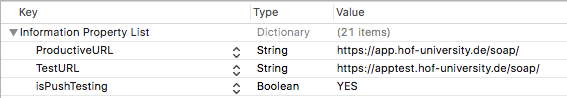
\includegraphics[width=0.9\textwidth]{plist} }
	\caption{Anpassungen in der Info.plist}
	\label{plist}
\end{figure}


Das Developer Team muss wie folgt ausgewählt werden, damit Push Notifications zur Verfügung stehen:
\begin{figure}[ht]
	\centering
  \frame{ 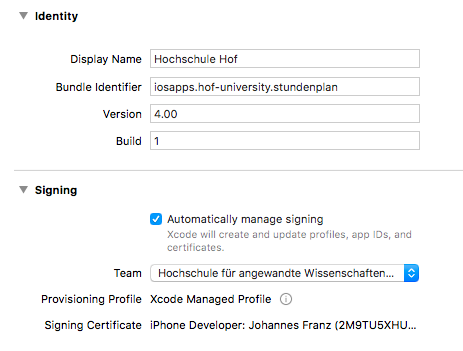
\includegraphics[width=0.9\textwidth]{devteam} }
	\caption{Wahl des Developer Teams}
	\label{devteam}
\end{figure}


Capabilities müssen wie folgt angepasst werden:

\begin{figure}[ht]
	\centering
  \frame{ 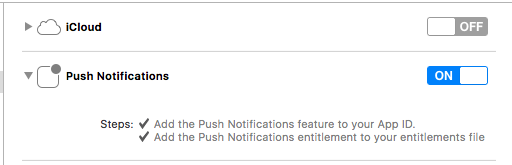
\includegraphics[width=0.9\textwidth]{capabilities} }
	\caption{Angepasste Capabilities}
	\label{capabilities}
\end{figure}



\section{Aufgetretene Probleme}
Als Herausforderung zu sehende Punkte haben häufig sehr viel Zeit in Anspruch genommen oder den Projektfortschritt entschleunigt.


\begin{itemize}
\item Verzögerte Bereitstellung des Servers führte zu komplexen Reimplementierungen in schwer zu synchronisierenden getrennten VMs
\item Beschränkte Rechte auf dem Testserver die nach und nach erweitert werden mussten
\item Verschiedene Zertifikatarten sind sehr verwirrend
\item Bundle Identifier und App Capabilities mussten nach jedem Git Pull wieder angepasst werden
\item Komplexes Testen (Lokale Server, Erreichbarkeit im Labornetzwerk / Wi-Fi, unterschiedliche Datei- und Serverstände) 
\item Zu Beginn kein Zugriff auf die Git Schnittstellen Projekt
\item Ablaufende Zertifikate
\item Serverseitig unterschiedliche Übertragungsverfahren zwischen Android und iOS
\item Erschwertes Debugging der PHP Scripte
\item HTTP2 wurde von Apache2 und Curl nicht offiziell unterstützt
\item Struktur der Datenbank und der PHP Scripte war durch die Android App vorgegeben
\item Veraltete APNs Variante war stark verbreitet, brachte allerdings viele Probleme mit sich und musste als Ansatz letztendlich verworfen werden
\end{itemize}


\section{Fazit}
Unser Team hat feststellen müssen, dass zu einem umfassenden iOS Projekt mehr als nur der Interface Builder und die Sprache Swift gehört. So sind Punkte zu nennen die positiv aus dem Projekt mitgenommen wurden.
\begin{itemize}
\item Linuxkenntnisse
\item PHP und Debugging auf dem Server
\item Beachten von Abhängigkeiten wie der Abwärtskompatibilität der Software zu früheren und bestehenden Android Versionen
\end{itemize}

\section{Weitere Arbeiten}
In diesem Projektabschnitt konnten alle gesteckten Ziele erreicht werden. Da solch ein relativ junges Projekt noch viele Möglichkeiten beinhaltet Funktionen zu verbessern und neue Funktionen einzuführen werden hier mögliche Punkte zur Anregung aufgelistet.

\begin{itemize}
\item Auswertungen die aktuell bei der Android und iOS App mehrfach auf dem Client Gerät stattfinden, können auf dem Server zentral bearbeitet werden. Dies verringert die Komplexität bei beiden Anwendungen und erleichtert die Wartung des Codes an zentraler Stelle.
\item Erweiterung der Push Notification Information um eine Priorität, Ablaufdatum,...
\item Aufkommende Issues und Ideen aus dem öffentlichen Git Projekt der iOS App und Schnittstelle
\item Erweiterung der App und Schnittstelle um andere Sprachen wie z.B. Englisch was in der Android App bereits angeboten wird

\end{itemize}

